\section[Udviklingsmetode]{Udviklingsmetode}

% Emneoverskrift. Start jeres del med denne:
\begin{frame}
  \frametitle{}
  \begin{center}
    {\Huge Udviklingsmetode}
  \end{center}
\end{frame}
\note{
  \begin{itemize}
		\item Notes...
  \end{itemize}
}

% Indhold:
\begin{frame}
    \frametitle{Udviklingsmetode i vores gruppe}
    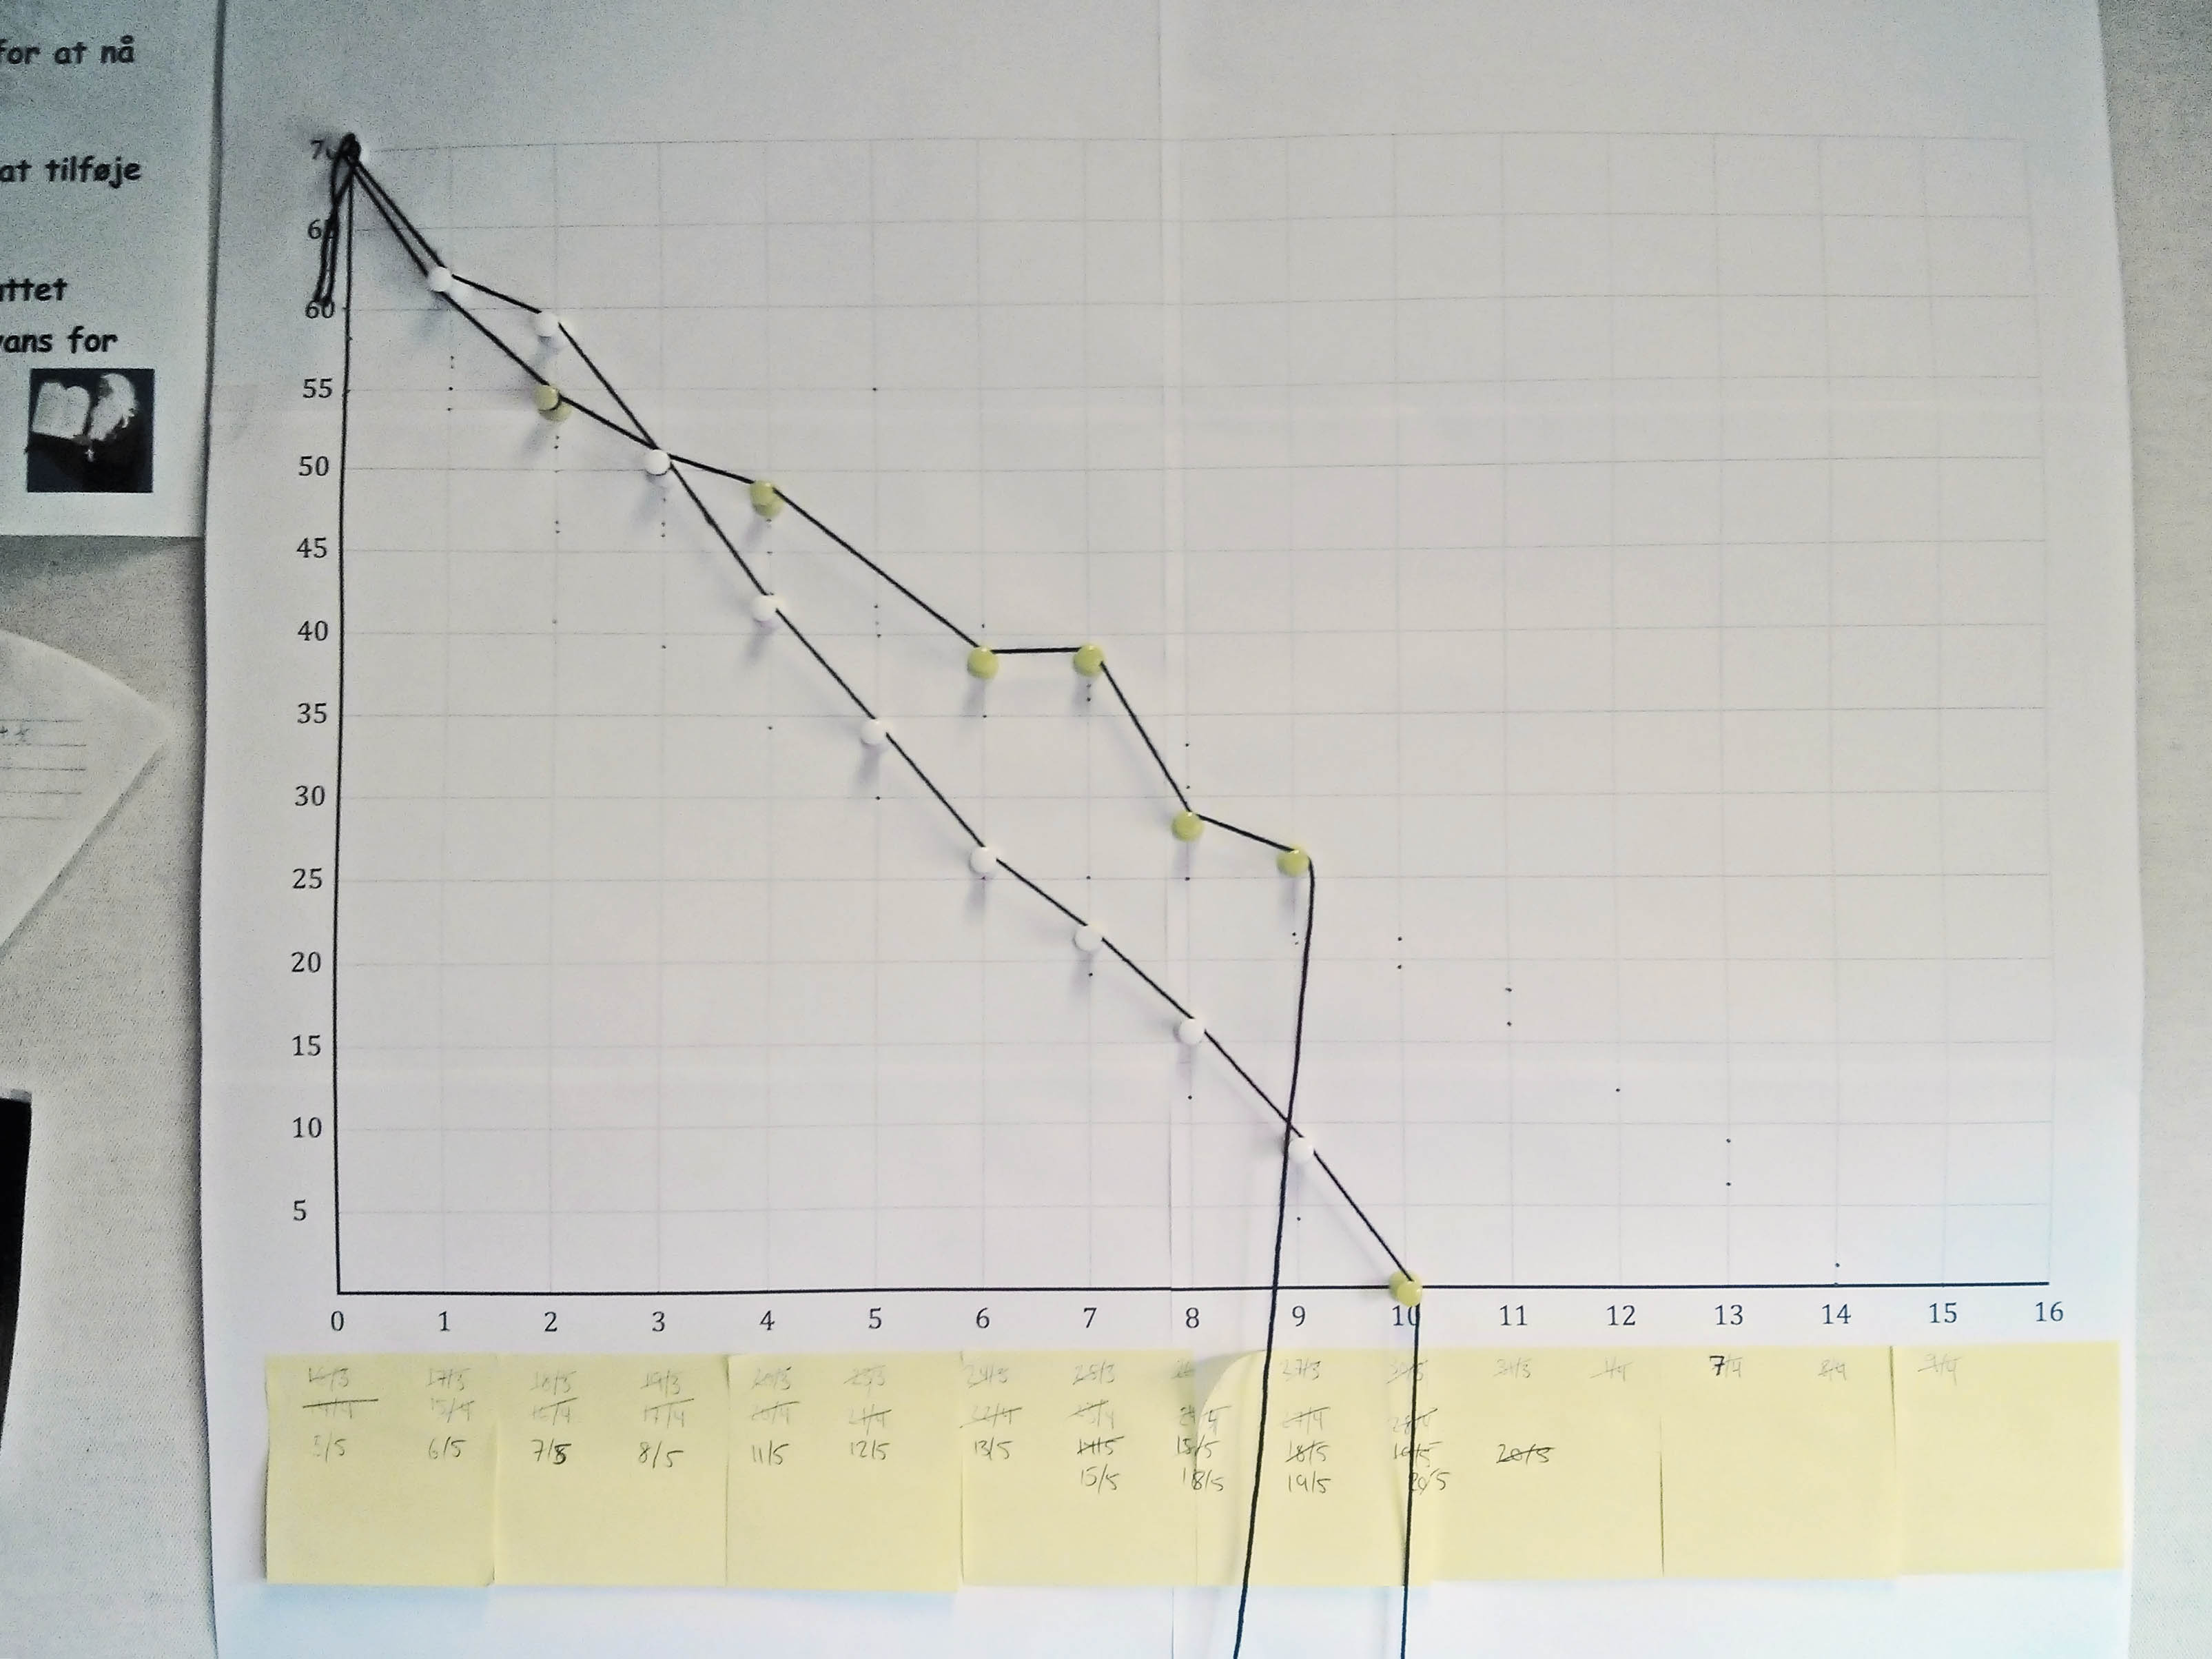
\includegraphics[width=0.48\textwidth]{burndown}~~~~
    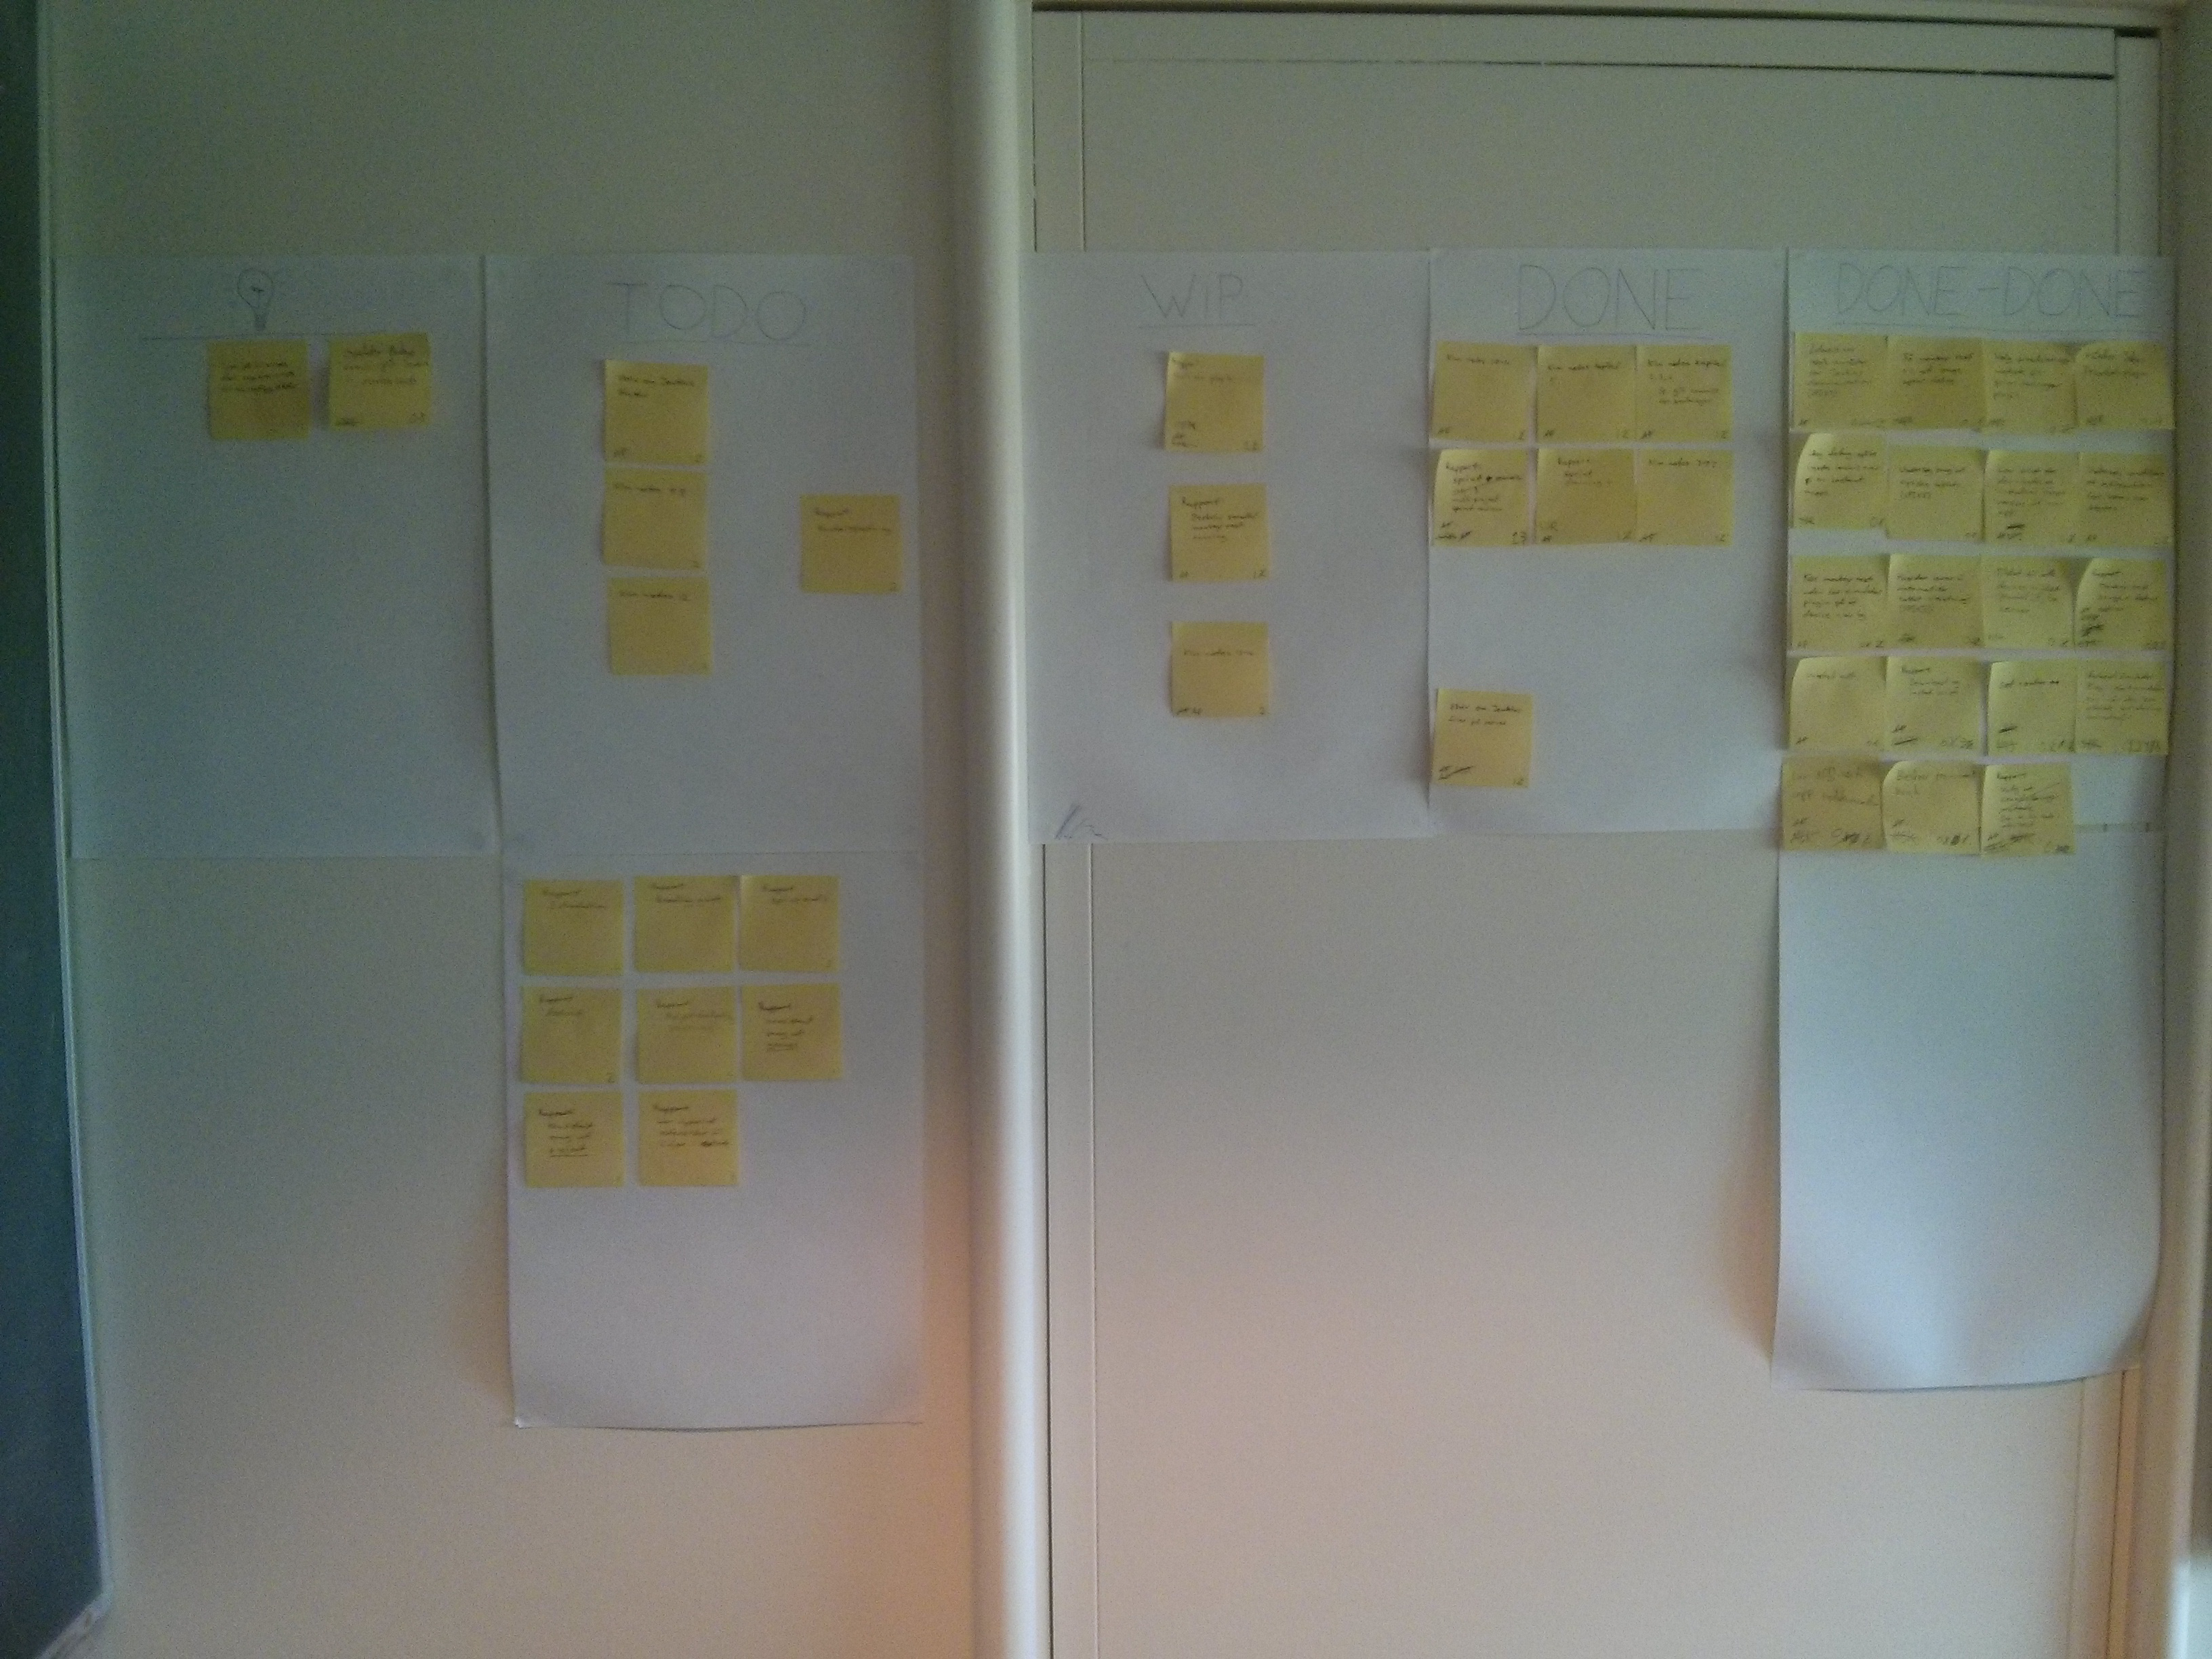
\includegraphics[width=0.48\textwidth]{kanban}
    
\end{frame}
\note{
	\begin{itemize}
		\item Scrum
    \item Det passer godt ind i multiprojektet.
    \item Daily Scrum
    \begin{itemize}
      \item Vælger opgaver fra sprint backloggen
      \item Opdaterer burndown
    \end{itemize}
    \item Scrumboardet (kanban): valgte backlog items > opsplitning i opgaver > planning poker. Enhed: halvdage. 
    \item Derudover følger vi udvkl.metode i multiprojektet.
    \item TODO: Hvad gør vi, når vi, som på billedet, er bagefter?
	\end{itemize}
}

\begin{frame}
    \frametitle{Udviklingsmetode i multiprojektet}
    \centering
    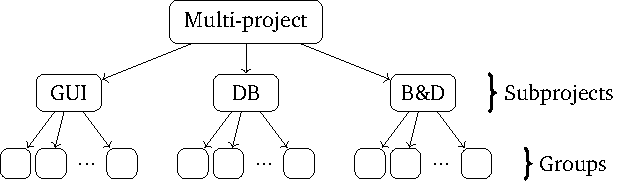
\includegraphics[width=0.8\textwidth]{multiproject_illustration.pdf}
\end{frame}
\note{
	\begin{itemize}
    \item 15 grupper, 3 subprojekter.
    \item En agil metode er et godt valg: ingen udviklererfaring med kode+krav+kunder, og vi har ikke tid til at analysere og forstå den nuværende kodebase. Vi skal bruge tiden på at få den til at virke!
    \item Figur:
    \begin{itemize}
      \item Multiprojekt-niveau: Sikre sig at roller, arbejdet og møderne overholdes. 1 ugentligt møde
      \item Subprojekt: Sprint planning, sprint review. Derudover 2-3 møder pr. uge.
      \item Gruppe: Scrum of (Scrums-something). Grupperne skal implementere interfacet Scrum. Hvad de gør, er vi ligeglade med.
    \end{itemize}
	\end{itemize}
}

\begin{frame}
    \frametitle{Udviklingsmetode i multiprojektet --- backlogs}
    \centering
    TODO: grafik med arbejdsprodukter.
\end{frame}
\note{
	\begin{itemize}
    \item Product backlog: Kundernes krav og ønsker.
    \item Release backlog: Nogle af disse ønsker flyttes over i en release backlog, og der arbejdes på dem i nuværende sprint.
	\end{itemize}
}

\begin{frame}
    \frametitle{Udviklingsmetode i multiprojektet}
    \centering
    TODO: grafik med backlog items.
\end{frame}
\note{
	\begin{itemize}
    \item Feature
    \item Bug
    \item Constraint
    \item Knowledge Acquisition
    \item Technical Work
    \item As a <type of user>, I want <some goal> so that <some reason>.
	\end{itemize}
}

\begin{frame}
    \frametitle{Udviklingsmetode i multiprojektet --- roller}
    \centering
    TODO: grafik med roller.\\
    
    \vspace{.6cm}
    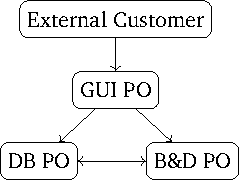
\includegraphics[width=0.4\textwidth]{po_illustration.pdf}
\end{frame}
\note{
	\begin{itemize}
    \item Scrum master: os.
    \item Product owner: Har kontakten med kunderne. 
	\end{itemize}
}

\begin{frame}
    \frametitle{Udviklingsmetode i multiprojektet --- møder}
    \centering
    TODO: grafik med møder.\\
\end{frame}
\note{
	\begin{itemize}
    \item TODO
	\end{itemize}
}


%%%%%%%%%%%%%%%%%%%%%%%%%
%% SCM
%%%%%%%%%%%%%%%%%%%%%%%%%
\begin{frame}
  \frametitle{}
  \begin{center}
    {\Huge Konfigurationsstyringsplan}
  \end{center}
\end{frame}
\note{
  \begin{itemize}
		\item Vigtig at identificere hvilke ting der skal styres, hvem de styres af, og hvilke redskaber man bruger til at styre dem med.
    \item Org. context:
    \item Unik struktur. Vi ønsker at tilfredsstille kunden, men har også andre prioriteter såsom gode, indholdsrige emner, så rapport og karakter også plejes. Vi har desuden ingen autoritet over andre grupper. 
  \end{itemize}
}

\begin{frame}
    \frametitle{Under Konfigurationsstyring}
    \begin{itemize}
      \item Kundernes krav
      \item Udgivne apps
      \item Udgivne biblioteker
      \item Gradle og Android Studio
      \item Kildekode
      \item Dokumentation af kildekode
    \end{itemize}
\end{frame}
\note{
	\begin{itemize}
      \item Kundernes krav: styres af produktejer
      \item Udgivne apps: 
      \item Udgivne biblioteker
      \item Gradle og Android Studio
      \item Kildekode
      \item Dokumentation af kildekode
	\end{itemize}
}

\begin{frame}
    \frametitle{Continuous Integration}
    \begin{itemize}
      \item Automatisk testning af apps og biblioteker
      \item Hyppig indfletning med master branch
      \item Nyeste dokumentation
      \item Automatisk kørsel af statiske analyser
    \end{itemize}
\end{frame}
\note{
	\begin{itemize}
    \item TODO
	\end{itemize}
}